%------------------------------------------------------------------------------
% SMURF Paper
%------------------------------------------------------------------------------

\documentclass[useAMS,usenatbib,nofootinbib]{mn2e}

% this is needed to get pdftex to work properly!
\usepackage[pdftex]{graphicx}

\usepackage{amsmath}
\usepackage{url}
\usepackage{natbib}
\usepackage{rotating}

% --- Some user defined macros ------------------------------------------------

% journals
\newcommand{\apj}{\rm ApJ}
\newcommand{\apjl}{\rm ApJL}
\newcommand{\apjs}{\rm ApJS}
\newcommand{\aaps}{\rm A$\&$AS}
\newcommand{\aap}{\rm A$\&$A}
\newcommand{\aapr}{\rm A$\&$AR}
\newcommand{\mnras}{\rm MNRAS}
\newcommand{\aj}{\rm Astron. J.}
\newcommand{\araa}{\rm ARAA}
\newcommand{\nat}{\rm Nature}
\newcommand{\pasj}{\rm PASJ}
\newcommand{\pasp}{\rm Publ. Astron. Soc. Pac.}
\newcommand{\ASP}{\rm ASP COnference Series}
\newcommand{\CASP}{\rm Comm. Astrophys. Space Phys.}
\newcommand{\astroph}{\rm astro-ph/}


% common acronyms etc.
\newcommand{\snr}{SNR}
\newcommand{\scuba}{SCUBA-2}
\newcommand{\rms}{RMS}

% these are approximately less-than and greater-than symbols
\def\lsim{\mathrel{\lower2.5pt\vbox{\lineskip=0pt\baselineskip=0pt
          \hbox{$<$}\hbox{$\sim$}}}}

\def\gsim{\mathrel{\lower2.5pt\vbox{\lineskip=0pt\baselineskip=0pt
          \hbox{$>$}\hbox{$\sim$}}}}


% ----------------------------------------------------------------------------

\title[SMURF: an iterative map-maker for SCUBA-2]{The Sub-Millimetre User
Reduction Facility: an iterative map-maker for SCUBA-2}

\author[Edward~L.~Chapin~et~al.]{
  \parbox[t]{\textwidth}{
    Edward~L.~Chapin$^{1}$\thanks{E-mail:~echapin@phas.ubc.ca},
    David~S.~Berry$^{2}$,
    Andrew~G.~Gibb$^{1}$,
    Tim~Jenness$^{2}$,
    Douglas~Scott$^{1}$
  }
  \\
  \\
  $^{1}$Dept. of Physics \& Astronomy, University of British Columbia,
  6224 Agricultural Road, Vancouver, B.C. V6T 1Z1, Canada\\
  $^{2}$JointAstronomy Centre, 660 N. A`oh\={o}k\={u} Place, University
  Park, Hilo, Hawaii 96720, USA}

\begin{document}

\label{firstpage}

\maketitle

\begin{abstract}
  We describe the properties of data from the Submillimetre Common
  User Bolometer Array 2 (SCUBA-2), and the production of maps using
  the Sub-Millimetre User Reduction Facility (SMURF).
\end{abstract}


\begin{keywords}
chicken, chicken: chicken, chicken: chicken -- chicken
\end{keywords}

%------------------------------------------------------------------------------
\section{Introduction}
\label{sec:intro}
%------------------------------------------------------------------------------

\textbf{Guideline for figures:}

\begin{itemize}
\item minimize excess whitespace around the figure to optimize usage of space
\item ensure a decent line thickness
\item use a Times font for labels with a thickness that resembles the
  text in the body. The font size should be similar to the main body
  text or larger
\item avoid using colour unless it is necessary for emphasis
\end{itemize}

\textbf{start intro here...}

The Submillimetre Common User Bolometer Array 2
\citep[\scuba,][]{holland2006} is a new instrument for the 15-m
James Clerk Maxwell Telescope (JCMT) on Mauna Kea, Hawai'i. The camera
can simultaneously image the sky in two broad bands centered over 450
and 850\,\micron. Ultimately, the instrument will also be equipped
with a Fourier transform spectrometer \citep[FTS-2,][]{gom2010}, and a polarimeter
\cite[POL-2,][]{bastien2005}. This paper describes the Submillimetre User Reduction Facility,
SMURF, a software package for reducing the imaging data, with an
emphasis on data taken during the SCUBA-2 Shared-Risks Observing period
(S2SRO) which took place from 2010 February 11 to 2010 March 25. The reduction
of FTS-2 and POL-2 data will be described at a later date once these
additional instruments have been commissioned.

Over the last twenty years, the submillimetre band (defined here to be
200--1000\,\micron) has revolutionized several important areas of
astrophysics: helping to characterize the early stages of
star-formation by identifying the dense, cold regions in molecular
clouds where stars may eventually form; discovering through blind
surveys the locations and surface density of a class of massive
star-forming galaxies in the early Universe, now referred to as
submillimetre galaxies, or SMGs; and finding debris disks around
nearby stars, the early stages of planet formation.

Styles of map-making: maximum likelihood
\citep[e.g.,][]{patanchon2008}; iterative -- see \citet{johnstone2000}
implementation of \citet{wright1996} to remove chop,
\citet{kovacs2008} for SHARC-2 etc.; de-correlation using PCA analysis
\citep[e.g.][]{laurent2005,scott2008,aguirre2010}.

Since \scuba\ will ultimately have nearly 10,000 working bolometers,
considerably larger than any other existing ground, or space-spaced
bolometer cameras, SMURF has been designed to use a less accurate,
though faster and less memory-intensive iterative approach that
attempts to model and remove most of the correlated signal components,
and then regrid the residuals signals. This method is similar in
spirit to the Comprehensive Reduction Utility for SHARC-2
\citep[CRUSH,][]{kovacs2008}, and the pipeline developed for the
Bolocam Galactic Plane Survey \citep{aguirre2010}.

%------------------------------------------------------------------------------
\section{Data Properties}
\label{sec:data}
%------------------------------------------------------------------------------

My thought is that this section would give the basics about how
SCUBA-2 works, and then more specific details for the S2SRO
observations.

%--------------------------------------------------
\subsection{How \scuba\ takes measurements}
%--------------------------------------------------

Before describing the data-reduction algorithm in detail, we summarize
the basic strategy used to make measurements with SCUBA-2.

The first generation of submm bolometer cameras used NTD germanium
thermistors (e.g., SCUBA, MAMBO, BOLOCAM, AzTEC, LABOCA...).
Generally speaking, these devices are operated using a current bias;
changing thermal conditions alter their impedence, resulting in a
changing Voltage that can be measured. The bolometers are cooled so
that they are {\em background limited} -- the dominant noise term is
the optical load from sources outside of the cryostat (emissivity from
telescope, atmospheric fluctuations, and astronomical sources).

In contrast, SCUBA-2 belongs to a new generation of cameras that uses
superconducting transition-edge sensors (TESs, like ACT, SPT,
MUSTANG). These devices are held at the critical temperature,
$T_\mathrm{C}$, below which the material becomes a superconductor, and
above which it becomes a normal conductor. Within this transition,
tiny temperature fluctuations can produce huge changes in
impedence. The devices are operated with a voltage bias, so that
thermal fluctuations produce changing currents, which in turn generate
changing local magnetic fields. Chains of superconducting quantum
interference devices (SQUIDs) are used to amplify these signals,
ultimately providing a larger changing current that may be
digitized. Like the NTD thermistor-based cameras, SCUBA-2 is cooled in
order to be background limited. However, a superior over-all
sensitivity on a per-bolometer basis is achieved through its improved
responsivity (similar to an improved quantum efficiency for a CCD).

The load on the detectors can vary substatially, both from thermal
sources within and outside the SCUBA-2 cryostat. In order to operate
the camera across a broad dynamic range of conditions, it is therefore
necessary to thermally control the focal plane. This is achieved by
providing a fridge {\em base temperature}, $T_\mathrm{B}$ that is
well-below $T_\mathrm{C}$, and then using heaters that are connected
to each bolometer to place the array in to transition.

The focal plane is divided into four quadrants, each filled with 32
column $\times$ 40 row sub-arrays labelled s4a--s4d at 450\,\micron,
and s8a--s8d at 850\,\micron. To avoid independent bias and readout
wires to each bolometer, each array is multiplexed by column. There is
an additional row of dark SQUIDs with no TESs or thermal absorber used
to monitor non-thermal noise sources.

The camera has been designed so that the absolute response of each
detector can be established by ramping currents through the individual
pixel heaters to produce Joule heating power, $P_\mathrm{J} =
\epsilon I^2R$, where $I$ is the known current, $R$ is the heater
resistance, and $\epsilon$ is the efficiency with which power is
transferred to the bolometer. In order to calibrate the total factor
$\epsilon R$, SCUBA-2 posesses an internal flatfield source.

For further detail see...

%-------------------------------------------------
\subsection{\scuba\ shared-risk observations}
%-------------------------------------------------

This paper will be focussed on S2SRO: only one subarray at each
wavelength; fridge oscillations; working detectors (and variation from
setup-to-setup).

Show some time series.

Show power spectra.

Show cross-spectra to emphasize how correlated things are?

\begin{figure}
\centering
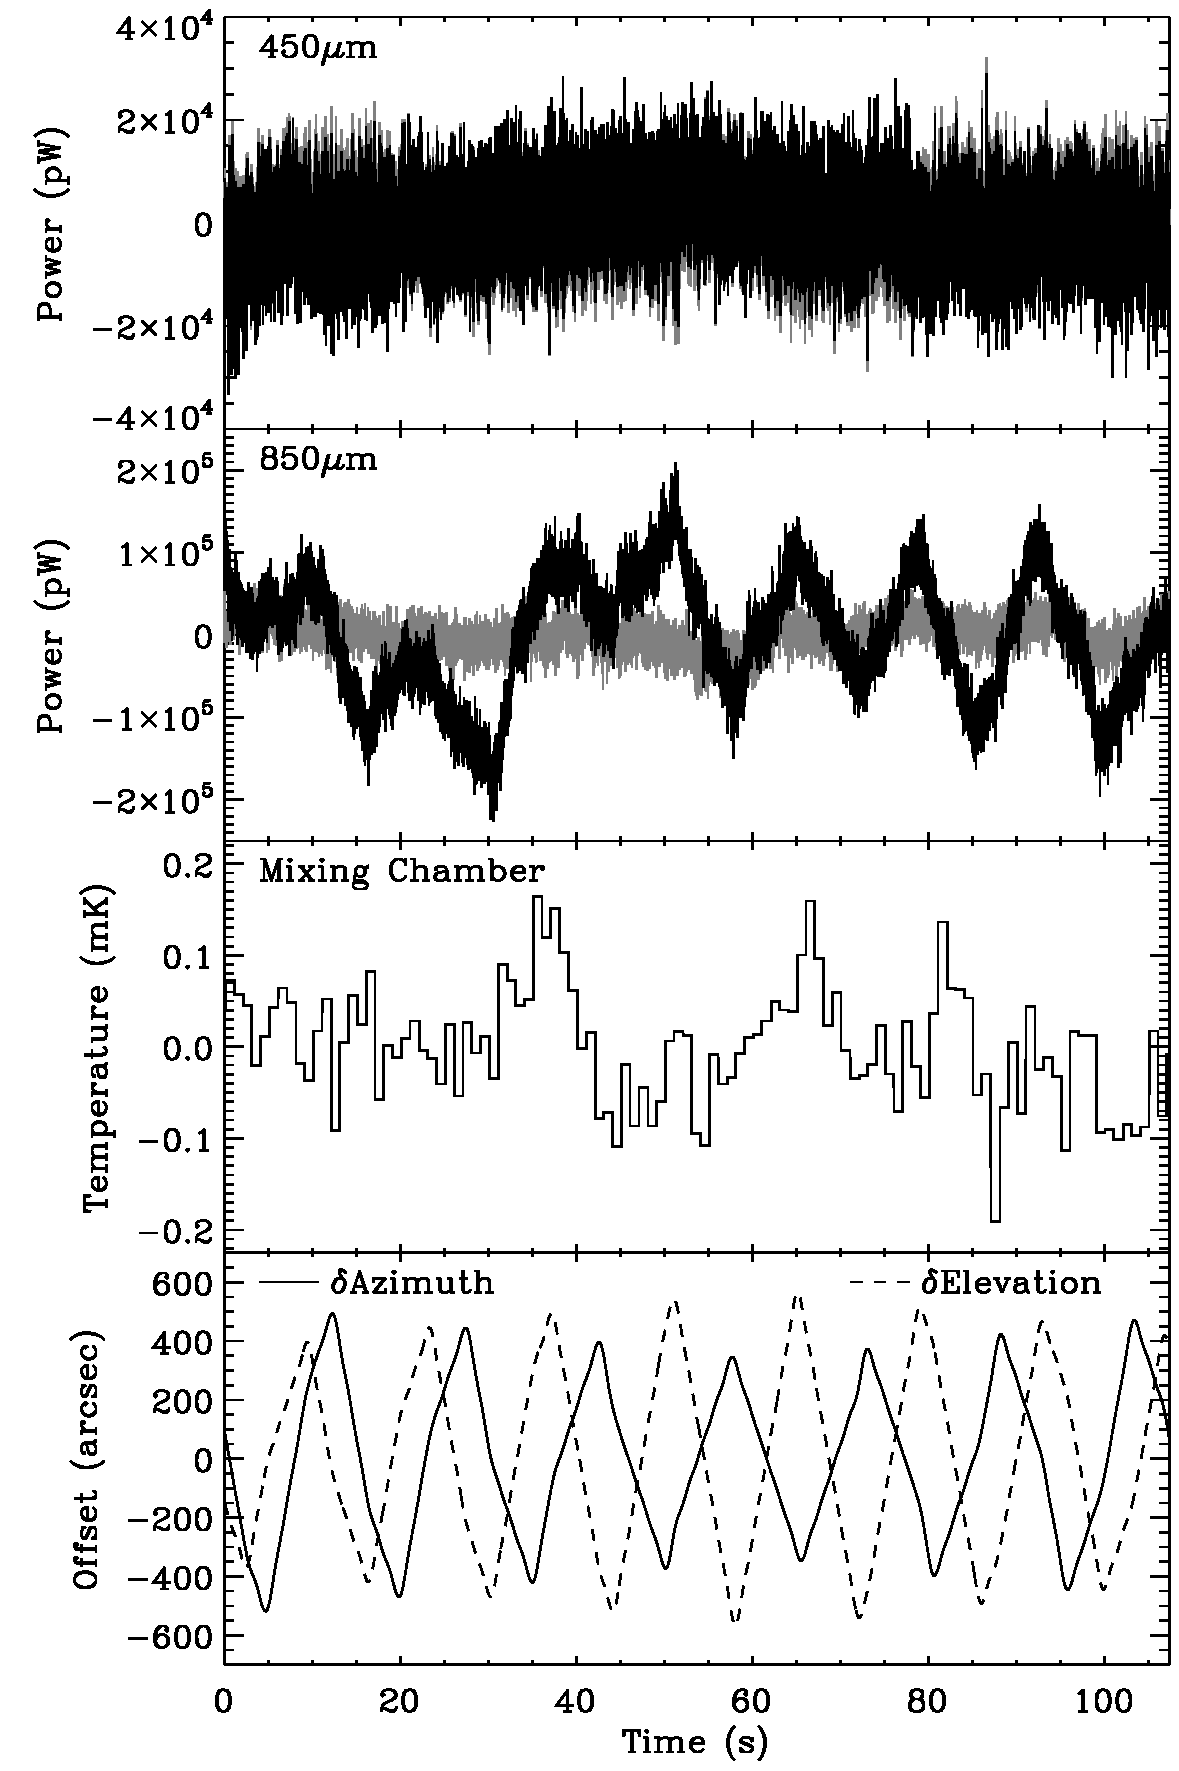
\includegraphics[width=\linewidth]{bolos_point_mix.pdf}
\caption{A comparison between single bolometer time series in each
  band (top two plots), with the mixing chamber temperature and
  azimuth/elevation pointing offsets. There is a strong correlation
  between the bolometers and the roughly $\sim$25\,s oscillation in
  the fridge, but not with the telescope motion. Also note that the
  total power in this primary signal is similar at both 450 and
  850\,\micron, pointing to an internal rather than an external
  source.}
\label{fig:bolos_mix}
\end{figure}

\subsubsection{Fridge oscillations}
As shown in Fig.~\ref{fig:bolos_mix}, the dominant signal in both
bands is clearly an oscillation in the fridge base temperature as
evidenced by the low-resolution mixing chamber thermometer. The total
power delivered to the bolometers is comparable at each wavelength,
further suggesting a source internal to the cryostat, rather than an
external optical load. Finally, there is no obvious correspondance
with either the azimuth or elevation motion.

Show what's left over when we remove the common-mode, and the
correlation of the resulting signal with patterns in $G$ and
$T_\mathrm{C}$ across the array.

\subsubsection{Sky noise}
Do we even see sky noise? Can show some results for the combined 450
and 850\,\micron\ joint PCA analysis.

\subsubsection{Magnetic field pickup}
Show that it occasionally appears in the dark squids.

\subsubsection{Line features}

The power spectra also show some narrower line features (many
correlated across the array). Even though we largely ignore them worth
some mention.

%------------------------------------------------------------------------------
\section{The SMURF Algorithm}
\label{sec:algorithm}
%------------------------------------------------------------------------------

Describe the bolometer signal model, and with the help of a flow-chart
show the basic procedure that SMURF follows.

We express the signal observed by the $i$th bolometer as a function of time,
\begin{equation}
\mathbf{b}_i(t) = g_i[\mathbf{e}_i(t) \mathbf{a}_i(t) + \mathbf{n}_i(t)]
\end{equation}
where $\mathbf{a}(t)$ is the time-varying signal produced by scanning
the telescope across astronomical sources, $\mathbf{e}(t)$ is the
time-varying extinction, which is a function of the telescope
elevation and atmospheric conditions, and $\mathbf{n}_i(t)$ represents
sources of noise. The two terms in square brackets, as written, have
units of power delivered to the detectors (pW). The scale factor $g_i$
converts this effective power to the digitized units recorded on disk
(DAC), and in this formulation is assumed to be constant in time.

In practice, $g_i$ is further factored into two components: $g_i = r_i
d$. The responsivity, $r_i$, gives the change in current as a function
of power fluctuations (A\,pW$^{-1}$). There is then a final (and
constant across all bolometers) conversion factor from current to DAC
units, $d$ (DAC/A).

As for the noise, $\mathbf{n}_i(t)$, we break it down into several
components,
%
\begin{equation}
  \mathbf{n}_i(t) = \mathbf{n}^\mathrm{w}_i(t) + \mathbf{n}^\mathrm{f}_i(t) +
  \mathbf{n}^\mathrm{c}(t),
\end{equation}
%
where $\mathbf{n}^\mathrm{w}_i(t)$ is uncorrelated white (thermal)
noise, $\mathbf{n}^\mathrm{f}_i(t)$ is low-frequency noise that is
\emph{not} correlated from bolometer-to-bolometer, and
$\mathbf{n}^\mathrm{c}(t)$ is a (predominantly low-frequency)
correlated or \emph{common-mode} component.

The primary goal of map-making is to model and remove
$\mathbf{n}^\mathrm{f}_i$ and $\mathbf{c}^\mathrm{f}_i$ from the
time-series. By re-gridding the remaining data we can then hope to
approach the theoretical noise limit in the map.

\begin{figure}
\centering
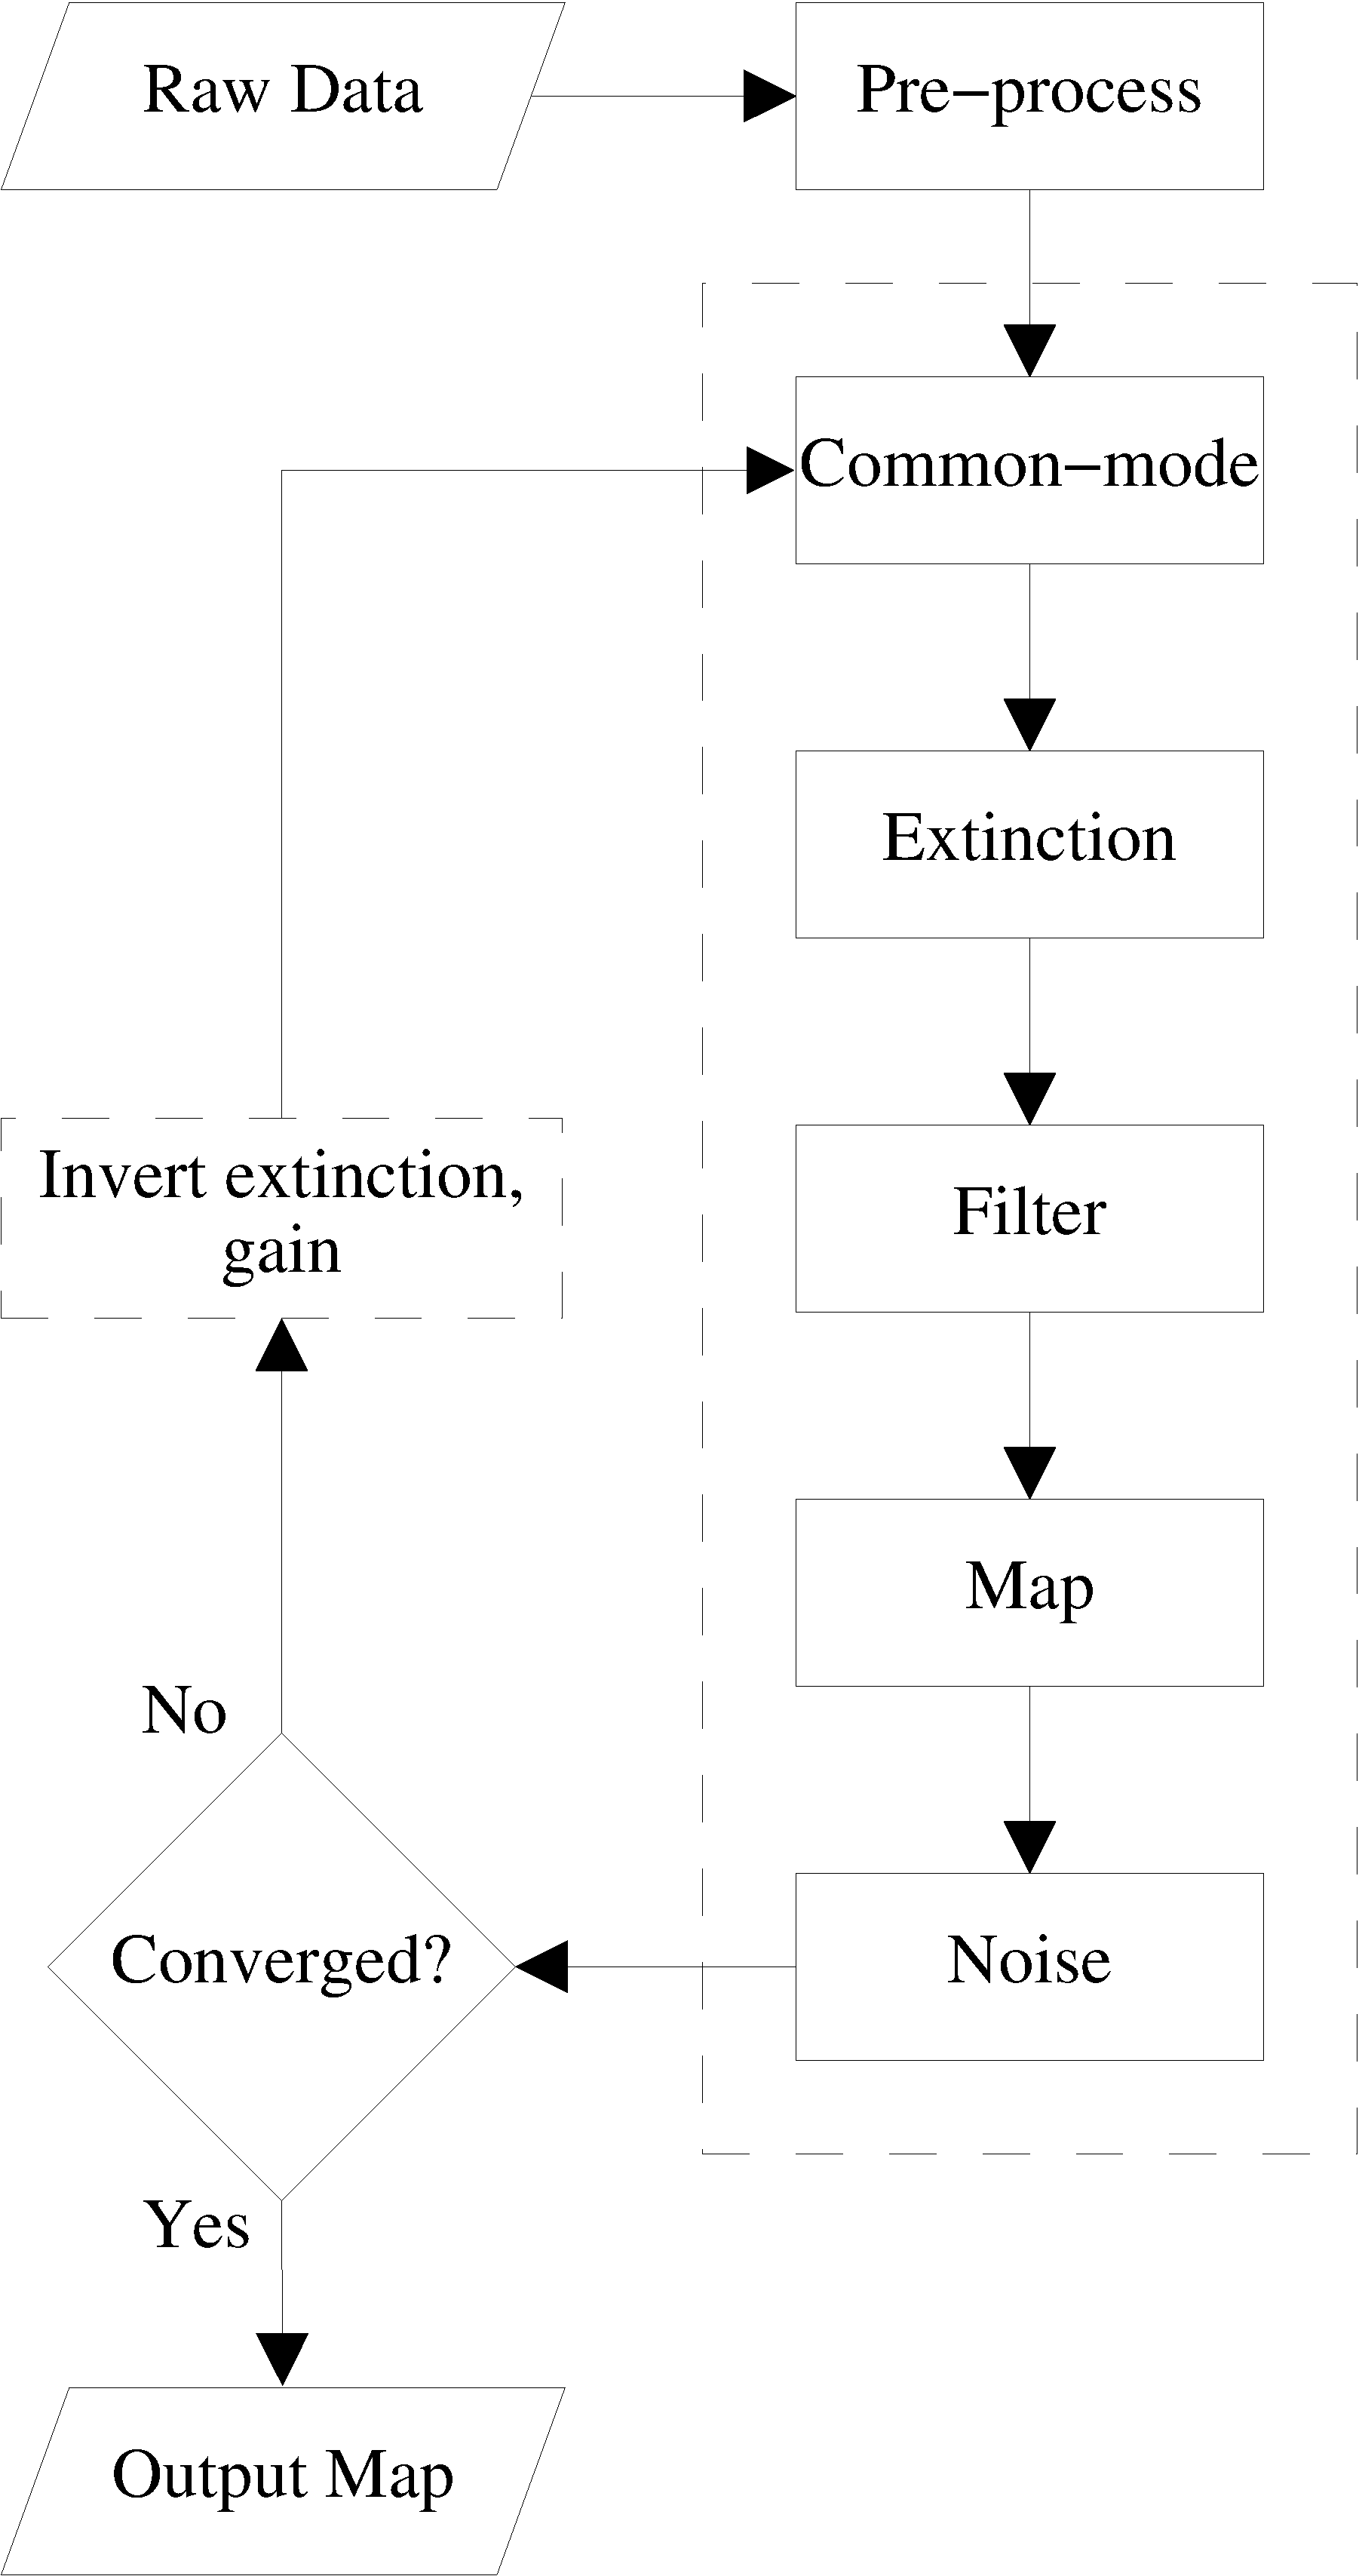
\includegraphics[width=0.75\linewidth]{dimm.pdf}
\caption{Typical map-making algorithm. Raw data (stored in multiple
  files) are read and concatenated into continuous time series. A
  pre-processing stage repairs DC steps, applies a flatfield
  correction, identifies and removes the noisiest bolometers, and
  flags large spikes. The iterative portion then begins: estimating
  and removing the common-mode signal; applying the extinction
  correction; high-pass filtering to remove residual independent
  low-frequency noise; estimating the map by re-gridding the data; and
  finally measuring the noise in the residual time series. If the
  \rms\ has converged, the final map is written to disk. Otherwise any
  multiplicative factors that may have been applied to the data are
  inverted (e.g., extinction correction and relative gains measured
  during the common-mode calculation), and each additive component is
  added back into the time series and re-estimated in turn.}
\label{fig:dimm}
\end{figure}

%-------------------------------------------------
\subsection{Model components}
%-------------------------------------------------

Give details about each model component, roughly in the order they are
calculated.

\subsection{Common-mode estimation}

DSB

We estimate the common-mode, remove it from the time series, use it to
flag bad bits of data, check for time-varying bolometer
responsivities... what doesn't it do?!

\subsection{Iterative filtering}

EC

The FFT filter can do high/low-pass filtering. We can also do notches
and whitening.

TJ

We also have the SMO median filter that's useful for very short scans
because edge effects don't matter so much.


\subsection{Noise estimation}

Measure a white noise level from the power spectrum for each detector
to use as a weight.

\subsection{Map estimation}

In the map, use weighted standard error to estimate noise. This is
accurate for a single pixel, but there is still spatially correlated
noise in the maps which we can show with some figures.

\subsection{Model degeneracies}

Introduce the topic of model degeneracies here, but defer their
solution to the example sections.

%-------------------------------------------------
\subsection{Data cleaning}
%-------------------------------------------------

Since we can do most of this stuff either as a pre-processing step or
iteratively, I thinks this goes in a generic-sounding subsection. This
can go here, or perhaps earlier?

\subsubsection{Time-domain de-spiking}

DSB

\subsubsection{Step correction}

DSB

\subsubsection{Gap filling / apodization}

DSB

Discuss gap filling, ``new'' window function method, also apodization
and start/end polynomial continuity stuff. Should reference CMB
literature (namely Stompor et al.).

\subsubsection{Flatfields}
\label{sec:flatfields}

TJ

Discuss heater ramps, normalizing off the common-mode signal
amplitude, astronomical sources, and the internal flatfield source.

\subsubsection{Additional bad bolometer rejection}

TJ

Measuring the noise power spectra and throwing away outliers. Data
flagged bad by the DA system.

\subsubsection{Map-based despiking}

EC

%------------------------------------------------------------------------------
\section{Examples}
\label{sec:examples}
%------------------------------------------------------------------------------

\subsection{Point source}
Reduce a calibrator. Describe the use of a zero mask around the
source. Compare with \citet{wiebe2009} who used the same method to
constrain a maximum-likelihood map with poor cross-linking.

\subsection{Deep blind survey}
Heavy initial filtering, and only iteratively solve for map and
common-mode with edge constraints.


\subsection{Bright extended emission}
The hardest thing to do with SCUBA-2 at the moment. Try to generate a
source/background mask to assist the map solution based on thresholds
in \snr. Compare with BOLOCAM stuff.

%------------------------------------------------------------------------------
\section{Summary and future work}
\label{sec:summary}
%------------------------------------------------------------------------------

\scuba\ is being re-commissioned. Maybe we will have some initial data
on fridge performance? If both it, and sky noise are relatively
well-behaved, might be able to restrict filtering to lower frequencies
and get larger-scale structures.

Larger array footprint also helps.

Talk about potential of Pascale et al. method to get closer to
max-likelihood map solution (handle maps at constant scan angles with
weights in Fourier space separately).

%------------------------------------------------------------------------------
\section{Acknowledgements}
%------------------------------------------------------------------------------


%------------------------------------------------------------------------------
\bibliographystyle{mn2e}
\bibliography{mn-jour,refs}
%------------------------------------------------------------------------------

%------------------------------------------------------------------------------
\appendix
\section[]{This is an appendix}
%------------------------------------------------------------------------------


\end{document}
